\documentclass[aspectratio=169,11pt]{beamer}
\usepackage[T1]{fontenc}
\usepackage{lmodern,amsmath,amssymb,mathtools,bm,booktabs,array,graphicx,tikz}
\usetikzlibrary{arrows.meta,positioning,calc,decorations.pathreplacing,patterns}
\definecolor{ink}{HTML}{17344D}\definecolor{accent}{HTML}{087E8B}\definecolor{pale}{HTML}{EDF5F5}\definecolor{gold}{HTML}{AD6B19}
\providecommand{\dd}{\,\mathrm{d}}\providecommand{\R}{\mathbb{R}}
\providecommand{\E}{\mathbb{E}}\providecommand{\Var}{\operatorname{Var}}
\providecommand{\Cov}{\operatorname{Cov}}\providecommand{\diag}{\operatorname{diag}}
\providecommand{\norm}[1]{\left\lVert#1\right\rVert}
\providecommand{\abs}[1]{\left|#1\right|}
\usefonttheme{professionalfonts}
\setbeamercolor{normal text}{fg=black,bg=white}
\setbeamercolor{frametitle}{fg=ink,bg=white}
\setbeamercolor{title}{fg=ink}\setbeamercolor{structure}{fg=accent}
\setbeamercolor{block title}{fg=ink,bg=pale}\setbeamercolor{block body}{fg=black,bg=pale!40}
\setbeamercolor{alerted text}{fg=accent}
\setbeamerfont{frametitle}{size=\Large,series=\bfseries}
\setbeamerfont{title}{size=\LARGE,series=\bfseries}
\setbeamertemplate{navigation symbols}{}
\setbeamersize{text margin left=.7cm,text margin right=.7cm}
\setbeamertemplate{frametitle}{\vspace{.18cm}\insertframetitle\par\vspace{.1cm}{\color{accent}\hrule height .6pt}\vspace{.12cm}}
\newcommand{\notestarget}{notes.pdf}\newcommand{\noteslabel}{Notes}
\setbeamertemplate{footline}{\hspace{.7cm}\color{ink}\scriptsize Mathematical Cardiology\quad\href{\notestarget}{\noteslabel}\hfill\insertframenumber\,/\,\inserttotalframenumber\hspace{.7cm}\vspace{.18cm}}
\setbeamercovered{invisible}
\hypersetup{pdfauthor={Zan Ahmad},pdftitle={Parallel circulation, shunt flow, and oxygen delivery},pdfpagemode=UseNone}
\begin{document}
\begin{frame}[plain]\vfill
{\small\color{accent} Mathematical Cardiology \quad Lecture 5}\par\medskip
{\raggedright\hyphenpenalty=10000\exhyphenpenalty=10000\LARGE\bfseries\color{ink} Parallel circulation, shunt flow, and oxygen delivery}\par\bigskip
Zan Ahmad\par\smallskip
{\small Fall 2023}\par\vfill\end{frame}
\renewcommand{\notestarget}{notes.pdf\#note-topology-comes-before-the-flow-calculation}
\begin{frame}[label=slide-serial-and-parallel-routes-figure]{Serial and parallel routes}
\centering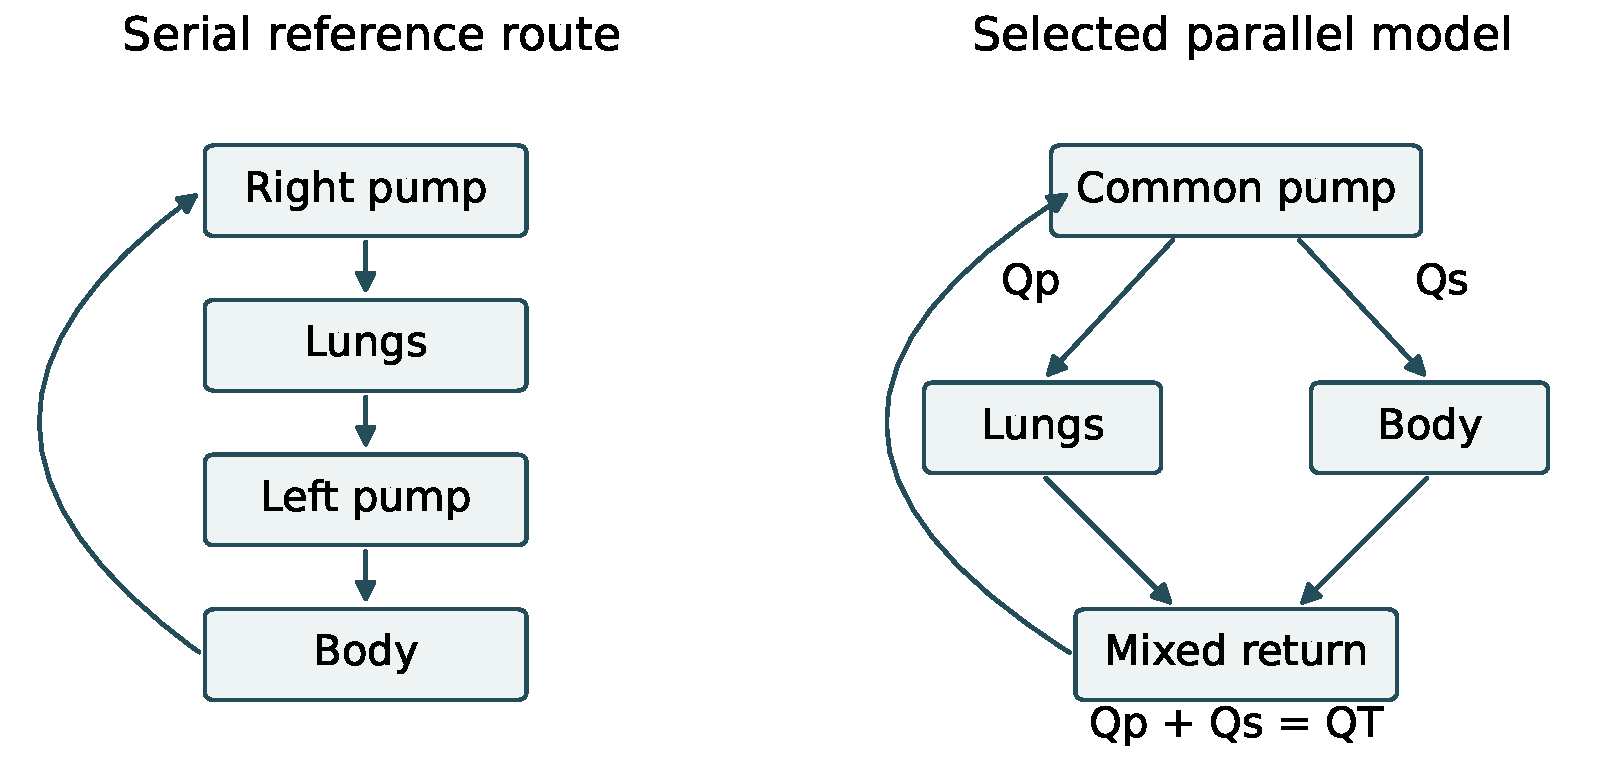
\includegraphics[width=.98\linewidth,height=.69\textheight,keepaspectratio]{circulation-routes.pdf}\end{frame}
\renewcommand{\notestarget}{notes.pdf\#note-topology-comes-before-the-flow-calculation}
\begin{frame}[t,fragile,label=slide-serial-and-parallel-routes]{Serial and parallel routes}
Series: one sustained flow traverses successive beds.\pause{}\par Parallel: the total flow divides among branches.\pause{}\par The selected parallel abstraction is not a Fontan model.
\end{frame}
\renewcommand{\notestarget}{notes.pdf\#note-topology-comes-before-the-flow-calculation}
\begin{frame}[t,fragile,label=slide-a-shunt-sign-convention]{A shunt sign convention}
\[Q_h=\frac{P_a-P_b}{R_h}.\]\pause{}\[\frac{12-8}{2}=2,\qquad\frac{8-12}{2}=-2\quad\mathrm{L/min}.\]\pause{} The chosen arrow defines positive flow.
\end{frame}
\renewcommand{\notestarget}{notes.pdf\#note-solve-the-parallel-flow-equations}
\begin{frame}[t,fragile,label=slide-three-equations-for-a-parallel-split]{Three equations for a parallel split}
\[Q_p=\Delta P/R_p,\qquad Q_s=\Delta P/R_s.\]\pause{}\[Q_p+Q_s=Q_T.\]
\end{frame}
\renewcommand{\notestarget}{notes.pdf\#note-solve-the-parallel-flow-equations}
\begin{frame}[t,fragile,label=slide-eliminate-the-branch-flows]{Eliminate the branch flows}
\[Q_T=\Delta P\left(\frac1{R_p}+\frac1{R_s}\right).\]\pause{}\[\Delta P=Q_T\frac{R_pR_s}{R_p+R_s}.\]
\end{frame}
\renewcommand{\notestarget}{notes.pdf\#note-solve-the-parallel-flow-equations}
\begin{frame}[t,fragile,label=slide-the-opposite-resistance-in-the-numerator]{The opposite resistance in the numerator}
\[Q_p=Q_T\frac{R_s}{R_p+R_s},\qquad Q_s=Q_T\frac{R_p}{R_p+R_s}.\]\pause{}\[\frac{Q_p}{Q_s}=\frac{R_s}{R_p}.\]
\end{frame}
\renewcommand{\notestarget}{notes.pdf\#note-solve-the-parallel-flow-equations}
\begin{frame}[t,fragile,label=slide-check-both-laws-and-conservation]{Check both laws and conservation}
\[Q_T=5,\quad R_p=10,\quad R_s=15.\]\pause{}\[Q_p=3,\quad Q_s=2,\quad \Delta P=30.\]\pause{}\[3+2=5,\qquad10(3)=15(2)=30.\]
\end{frame}
\renewcommand{\notestarget}{notes.pdf\#note-mix-contents-by-conserving-oxygen}
\begin{frame}[t,fragile,label=slide-oxygen-content-has-a-transport-unit]{Oxygen content has a transport unit}
\[[C]=\mathrm{mL\ O_2/L\ blood}.\]\pause{}\[[QC]=\mathrm{mL\ O_2/min}.\]\pause{} Content is not saturation or partial pressure.
\end{frame}
\renewcommand{\notestarget}{notes.pdf\#note-mix-contents-by-conserving-oxygen}
\begin{frame}[t,fragile,label=slide-mixing-is-an-oxygen-balance]{Mixing is an oxygen balance}
\[Q_TC_m\Delta t=Q_pC_p\Delta t+Q_sC_s\Delta t.\]\pause{}\[C_m=\frac{Q_pC_p+Q_sC_s}{Q_T}.\]
\end{frame}
\renewcommand{\notestarget}{notes.pdf\#note-mix-contents-by-conserving-oxygen}
\begin{frame}[t,fragile,label=slide-the-numerical-mixture]{The numerical mixture}
\[Q_pC_p=3(200)=600,\quad Q_sC_s=2(120)=240.\]\pause{}\[C_m=\frac{600+240}{5}=168\ \mathrm{mL\ O_2/L}.\]
\end{frame}
\renewcommand{\notestarget}{notes.pdf\#note-mix-contents-by-conserving-oxygen}
\begin{frame}[t,fragile,label=slide-why-the-mixture-lies-between-its-inputs]{Why the mixture lies between its inputs}
Let $x=Q_p/Q_T$, with $0\le x\le1$.\pause{}\[C_m=xC_p+(1-x)C_s.\]\pause{} The weights are nonnegative and sum to one.
\end{frame}
\renewcommand{\notestarget}{notes.pdf\#note-content-and-delivery-enter-as-a-product}
\begin{frame}[t,fragile,label=slide-delivery-uses-systemic-flow]{Delivery uses systemic flow}
\[D_s=Q_sC_m=2(168)=336\ \mathrm{mL\ O_2/min}.\]\pause{} Delivery entering a bed differs from consumption within it.
\end{frame}
\renewcommand{\notestarget}{notes.pdf\#note-content-and-delivery-enter-as-a-product}
\begin{frame}[label=slide-lower-only-pulmonary-resistance-figure]{Lower only pulmonary resistance}
\centering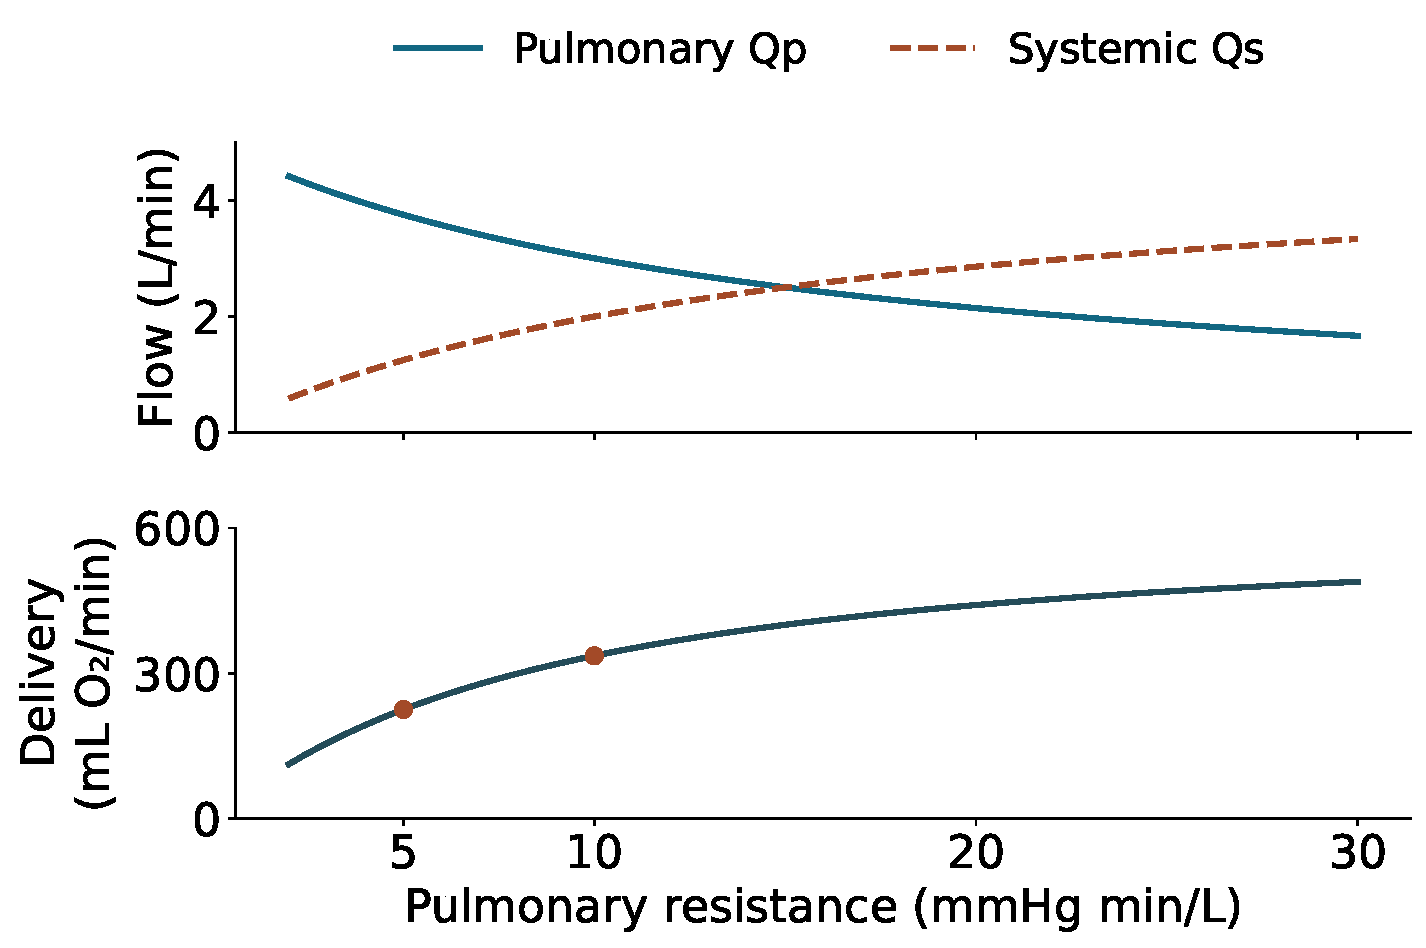
\includegraphics[width=.98\linewidth,height=.69\textheight,keepaspectratio]{flow-and-delivery.pdf}\end{frame}
\renewcommand{\notestarget}{notes.pdf\#note-content-and-delivery-enter-as-a-product}
\begin{frame}[t,fragile,label=slide-lower-only-pulmonary-resistance]{Lower only pulmonary resistance}
\[R_p:10\to5\Rightarrow Q_p=3.75,\ Q_s=1.25.\]\pause{}\[C_m=180,\qquad D_s=1.25(180)=225.\]\pause{} Higher mixed content accompanies lower systemic delivery.
\end{frame}
\renewcommand{\notestarget}{notes.pdf\#note-content-and-delivery-enter-as-a-product}
\begin{frame}[t,fragile,label=slide-write-the-tradeoff-as-one-polynomial]{Write the tradeoff as one polynomial}
\[\frac{D_s}{Q_T}=(1-x)\{120+80x\}.\]\pause{}\[=120-40x-80x^2.\]
\end{frame}
\renewcommand{\notestarget}{notes.pdf\#note-content-and-delivery-enter-as-a-product}
\begin{frame}[t,fragile,label=slide-compare-two-pulmonary-fractions]{Compare two pulmonary fractions}
For $\delta>0$ and $x+\delta\le1$,\[\frac{D_s(x+\delta)-D_s(x)}{Q_T}=-40\delta-160x\delta-80\delta^2<0.\]\pause{} This conclusion uses the prescribed return contents.
\end{frame}
\renewcommand{\notestarget}{notes.pdf\#note-streaming-extraction-and-missing-oxygen-dynamics}
\begin{frame}[t,fragile,label=slide-close-the-accounting-then-challenge-the-assumptions]{Close the accounting, then challenge the assumptions}
Check equal branch drops, total blood flow, and oxygen-volume balance.\pause{}\par Then ask whether complete mixing and fixed return contents describe the intended system.
\end{frame}
\end{document}
